\subsection{Day 1} \label{sec:day1}

The daily meeting took place as planned at 11:00 \gls{PST}.

It was noted the transfer took longer than expected - a potential network problem was suspected.
The data transfer script has a 5 second delay which should have been removed which made the transfer take far too long.
To keep the process running the dataset, which was already at \gls{NCSA}, was copied in to the incoming folder.

This was ingested into \texttt{/project/OpsRehearsal\_1/night1}  and processing (\texttt{singleFrameDriver.py}) ran  smoothly  averaging  ~1.5 CCDs/s  (running with 24 cores x 3 nodes), taking a total of 48 minutes.


29 “FATAL” errors (w/58 Runtime Errors) were noted among the 1,997 CCDs processed
There were issues with N stars and \gls{PSF} build and  Flux limit (linked to a a known problem).

The odd number of CCDs (not multiple of 9) was immediately remarked upon and investigated.  

Morganson found it was  missing one exposure from the 01687569 series using :
\code{for exp in `ls | cut -c 1-8 | sort -u`; do nexp=`ls \$exp* | wc -l`; echo \$exp, \$nexp; done}
This was not a transfer problem the simulation was made with once \gls{CCD} missing in one exposure.

QA scripts were kicked off by MacArthur including \texttt{visualizeVisit.py}\footnote{\url{https://community.lsst.org/t/y-band-stray-light-correction-for-hsc/2517}}, the latter did not work and needed a \gls{patch}.
Plots were accessible \url{https://lsst-web.ncsa.illinois.edu/~lauren/OpsRehearsal_1/attempt1/plots/}.
Some “issues” became clear perusing some of the plots.  As an example, the upward tilt towards bright magnitudes in \figref{fig:bfp} is a red flag for the “Brighter Fatter” issue.


\begin{figure}
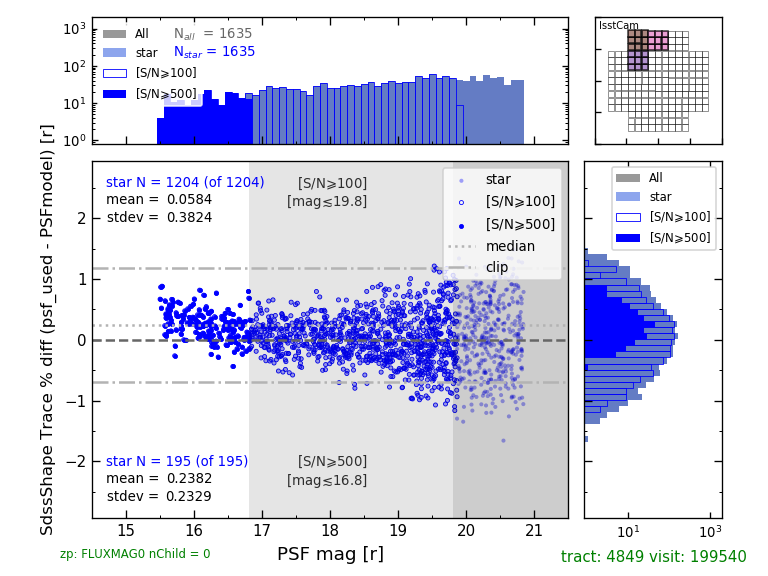
\includegraphics[width=0.8\textwidth]{plots/plot-v199540-psfTraceDiff-psfMagHist}
\caption{Brighter fatter effect evidence }
\label{fig:bfp}
\end{figure}



\subsubsection{Discussion}
We discussed how to implement change in code with tight turn around (need sign off from SciOps \gls{AD}).
How should one decide to rerun -  we need policies to affect or not nightly or daily changes in case of failures. Probably there is some percent level of problems we would accept, one percent seems ok two starts to seem a lot.  It was noted that problems stemming from a new software version should always have the possibility to revert to a previous stable version.

The need for some sort of rolled up \gls{QA} status were discussed - MacArthur came up with some summary files an example of which \texttt{visitAnalysis\_OpsRehearsal\_night1\_i.shortSum.txt} is in \appref{sec:visitsum}.

